\pdfoutput=1
\documentclass[aps,prd, amsmath,amssymb,superscriptaddress,showkeys,nofootinbib,reprint,preprintnumbers]{revtex4-1}
\usepackage{color}
\usepackage{aas_macros}
\usepackage{hyperref,breakurl}
\usepackage[usenames,dvipsnames]{xcolor}
\usepackage{dcolumn}
\usepackage{bm}
\usepackage{hyperref}
\usepackage{array}
\usepackage{dcolumn}

\usepackage{amsmath,amssymb,latexsym,times}
\DeclareMathOperator\arctanh{arctanh}

\usepackage{todonotes}
\newcommand{\verify}[1]{\textcolor{red}{\textbf{{#1}}}}

\newcommand\assign[1]{\todo[color=RoyalPurple!40, inline, size=\small]{Contributing: #1}}
\newcommand\troxel[1]{\todo[color=cyan!40, inline, size=\small]{Troxel: #1}}
 
\newcommand\green[1]{\textcolor{green}{#1}}

\begin{document}

\title{A synthetic WFIRST survey: Simulation suite and the impact of wavefront errors on weak lensing}

%\author{Troxel, M.A.}
%\email{michael.troxel@duke.edu}
\author{and others}

\collaboration{WFIRST HLS Cosmology SIT}

\noaffiliation

\date{\today}

\label{firstpage}

\begin{abstract}
\end{abstract}

\keywords{}

\maketitle

%\tableofcontents

\section{Introduction}\label{sec:intro}

\begin{itemize}
\item DE/cosmology context
\item motivation for WFIRST in context of other stage iii and stage iv surveys
\item cosmology sit
\item goals of paper
\end{itemize}


The nature of dark energy, which drives cosmic acceleration in the Universe, remains one of the most fundamental mysteries in physics twenty years after its discovery \cite{riess98,perlmutter99,detf,Frieman:2008sn,weinberg13}. 
A number of new experiments have been undertaken to probe dark energy using a variety of physical phenomena, including baryon acoustic oscillations, numbers and masses of galaxy clusters, galaxy clustering, redshift space distortions, Type Ia supernovae, and weak gravitational lensing. 
Current generation experiments are limited to some subset of these probes, but have already begun to expose interesting questions about the soundness of our standard cosmological model, Lambda-Cold Dark Matter (LCDM) that will require more and better data to resolve. 
The Wide-Field InfraRed Space Telescope (WFIRST) has been designed to take advantage of all of these probes to study dark energy with unprecedented systematic control \cite{2019BAAS...51c.341D,2019arXiv190205569A}.

In the past few years, the current generation of ground-based weak lensing experiments like the Dark Energy Survey (DES), Hyper-Suprime Cam (HSC), and Kilo-Degree Survey (KiDS) have reached levels of precision that rival the previously best possible cosmological constraints including dark energy \cite{}. 
These surveys have spurred the development of revolutionary algorithms and methods for galaxy shape measurement and weak lensing analysis \cite{}, highlighting the immense power of weak lensing to unravel the fundamental mysteries we face in cosmology today. 

By the planned launch of WFIRST in 2025, we will have final results from the ongoing generation of weak lensing experiments (DES, HSC, and KiDS) and preliminary results from the Dark Energy Spectroscopic Instrument (DESI), the Large Synoptic Survey Telescope (LSST), and the Euclid mission. 
Faced with the unknown discovery potential of these experiments in the early 2020s, it is vital to maintain the agility and flexibility of the WFIRST mission to respond with the best possible science, particularly in what is likely to be a systematics dominated weak lensing field.
The process of quantifying empirically the robustness of the design requirements of the WFIRST mission for weak lensing now in Phase B of the mission development is a critical task that this paper will attempt to address. 
Precise control of these systematics at the statistical precision offered by current WFIRST mission forecasts will enable WFIRST to play the likely role of arbiter in the study of new discoveries made in the early years of LSST and Euclid.

We present in this paper a set of synthetic WFIRST imaging surveys covering approx. 6 sq. deg. in one filter: a fiducial set of images and 11 variations in ways the PSF could be mis-estimated. 
It incorporates realistic distributions of photometric properties for galaxies and stars; complex analytic galaxy models; a simulated fiducial five year, 2000 sq. deg. observation strategy for the survey; and realistic detector effects, PSF models, and WCS solutions that match current (Cycle 7) design specifications. 
We use a blending-free version of this simulation to test the impact on weak lensing science of a variety of PSF or wave-front errors, including static, low-, and high-frequency biases. 

(insert standard toc para) 


\section{WFIRST and requirements}\label{sec:wfirst}
\assign{Hirata}

\begin{itemize}
\item What WFIRST is \& timeline
\item Previous requirements information
\item context in broader sit work
\item transition to empirical validation (next section)
\end{itemize}

\def\arraystretch{1.4}
\setlength{\tabcolsep}{4pt}
\begin{table}
\caption{Table}
\label{table:values}
\begin{center}
\begin{tabular}{lcccc }
\hline
\hline
%Parameter & $o$CDM & $w$CDM & $w$CDM (Ext) & Flat Prior \\ 
%\hline
%$\Omega_m$                                                  & $0.299^{+0.024}_{-0.020}$  &  $0.300^{+0.023}_{-0.021}$  & $0.303^{+0.007}_{-0.009}$ & [0.1, 0.9] \\
%$\Omega_b$                                                   & $0.069^{+0.009}_{-0.012}$   & $0.064^{+0.013}_{-0.009}$  & $0.048^{+0.001}_{-0.001}$ & [0.03, 0.12] \\
%$\Omega_k$                                                   & $0.252^{+0.095}_{-0.14}$     & 0 & 0 & [-0.1, 0.5] \\
%$\Omega_\Lambda$                                       & $0.47^{+0.14}_{-0.12}$        & $0.700^{+0.021}_{-0.023}$  & $0.697^{+0.009}_{-0.007}$ & Derived \\
%$w$                                                                 & $-1$                                      & $-0.80^{+0.09}_{-0.11}$       & $-1.02^{+0.03}_{-0.04}$ & [-2, -0.33] \\
%$S_8$  							    & $0.801^{+0.028}_{-0.026}$  & $0.786^{+0.029}_{-0.019}$   & $0.814^{+0.016}_{-0.011}$ & Derived \\ 
\hline
\hline
\end{tabular}
\end{center}
\end{table}

\begin{figure*}
\begin{center}
\includegraphics[width=\textwidth]{figures/fov.pdf}
\end{center}
\caption[]{
A simulated field-of-view (FOV) from the fiducial simulation matching Cycle 7 specifications. The WFIRST FOV is 0.282 deg$^2$, composed of 18 near-IR Sensor Chip Arrays (H4RGs). This FOV is 200 times the area of the Hubble Space Telescope Wide Field Camera 3 FOV and 90 times that of its Advanced Camera for Surveys. (check chip orientation)
\label{fig:fov}}
\end{figure*}

\begin{figure}
\begin{center}
\includegraphics[width=\columnwidth]{figures/sca1.png}
\end{center}
\caption[]{
A simulated WFIRST Sensor Chip Array (SCA). Each SCA (HgCdTe H4RG) has a useable pixel grid of 4088$\times$4088, with a pixel scale of 0.11''. One interesting feature can be seen in the relatively bright galaxy in the lower middle part of the SCA, for which six faint diffraction spikes due to the WFIRST secondary mirror support struts are visible.
\label{fig:sca}}
\end{figure}

\begin{figure}
\begin{center}
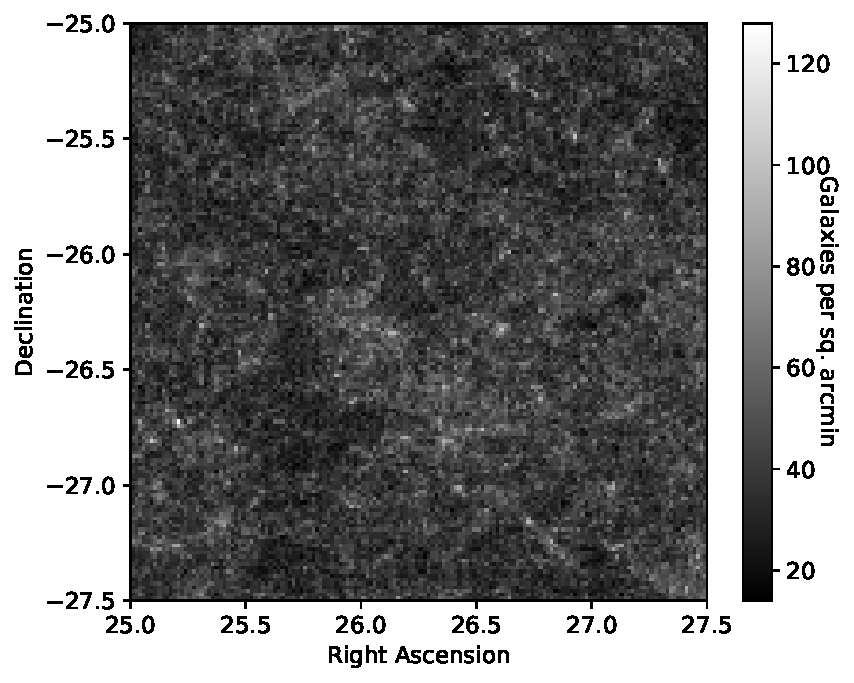
\includegraphics[width=\columnwidth]{figures/galaxies.pdf}
\end{center}
\caption[]{
The distribution of simulated galaxies. The mean galaxy density is 40 arcmin$^{-2}$. 
\label{fig:galaxies}}
\end{figure}

\begin{figure}
\begin{center}
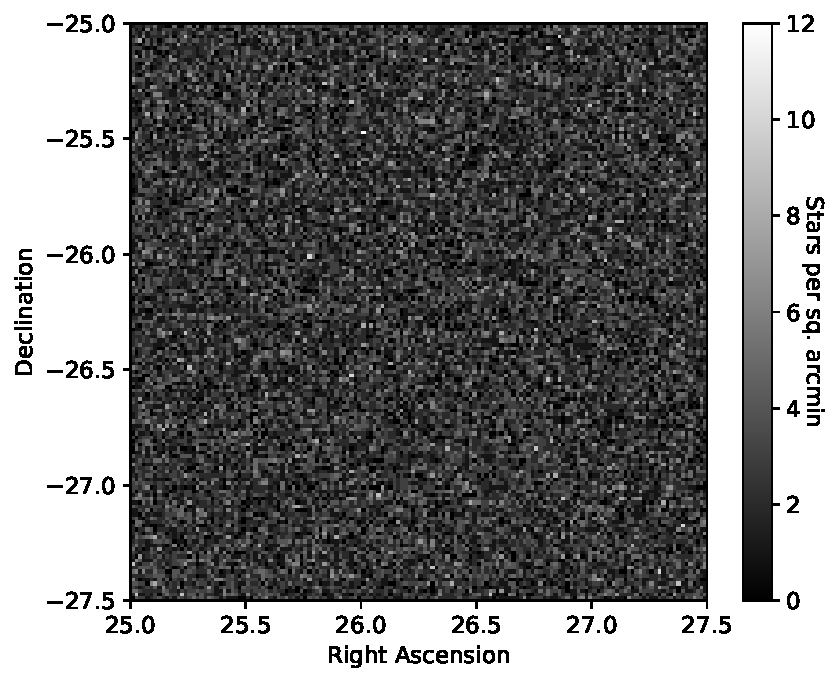
\includegraphics[width=\columnwidth]{figures/stars.pdf}
\end{center}
\caption[]{
The distribution of simulated stars. The mean stellar density is 2.5 arcmin$^{-2}$. 
\label{fig:stars}}
\end{figure}

\begin{figure*}
\begin{center}
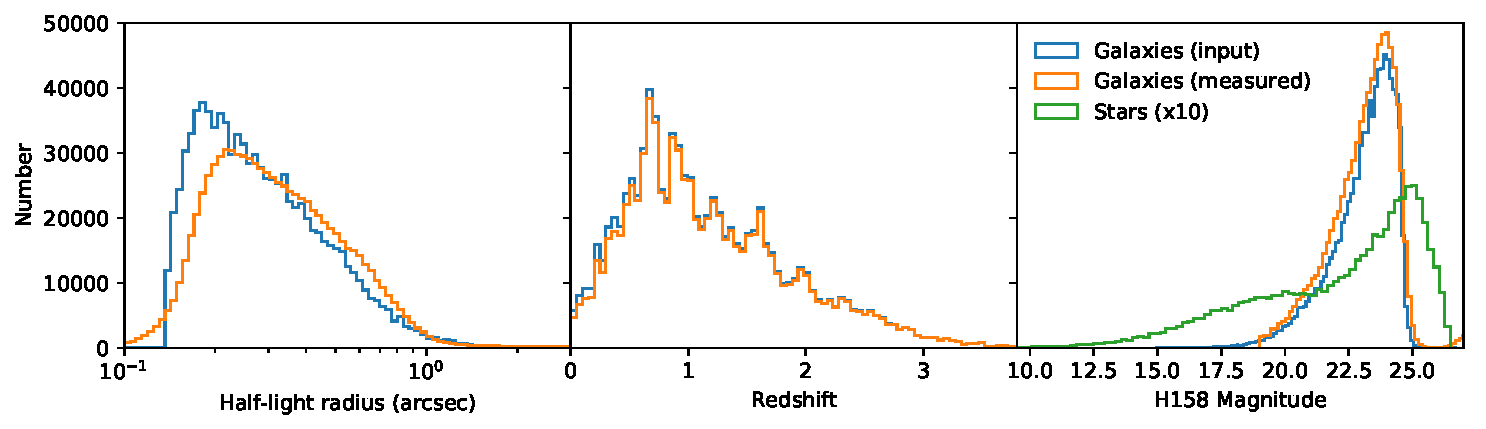
\includegraphics[width=\textwidth]{figures/hist.pdf}
\end{center}
\caption[]{
The input distributions of half-light radius, redshift, and H158 magnitude for galaxies (blue) and stars (orange).
\label{fig:hist}}
\end{figure*}

\begin{figure}
\begin{center}
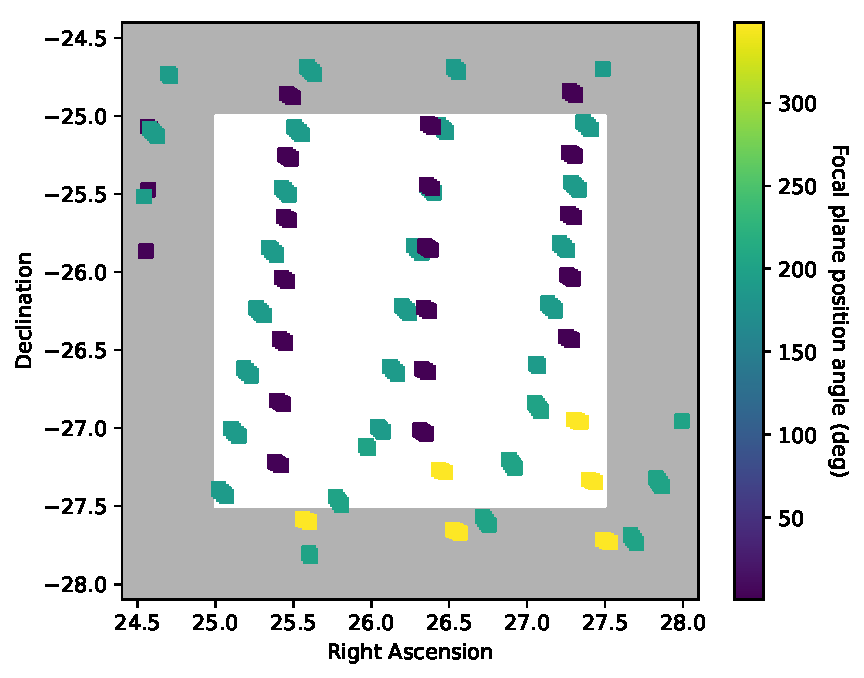
\includegraphics[width=\columnwidth]{figures/pointings.pdf}
\end{center}
\caption[]{
Pointings that overlap the simulated region (non-shaded). The color of each marker shows the position angle of the focal plane.
\label{fig:pointings}}
\end{figure}

\begin{figure*}
\begin{center}
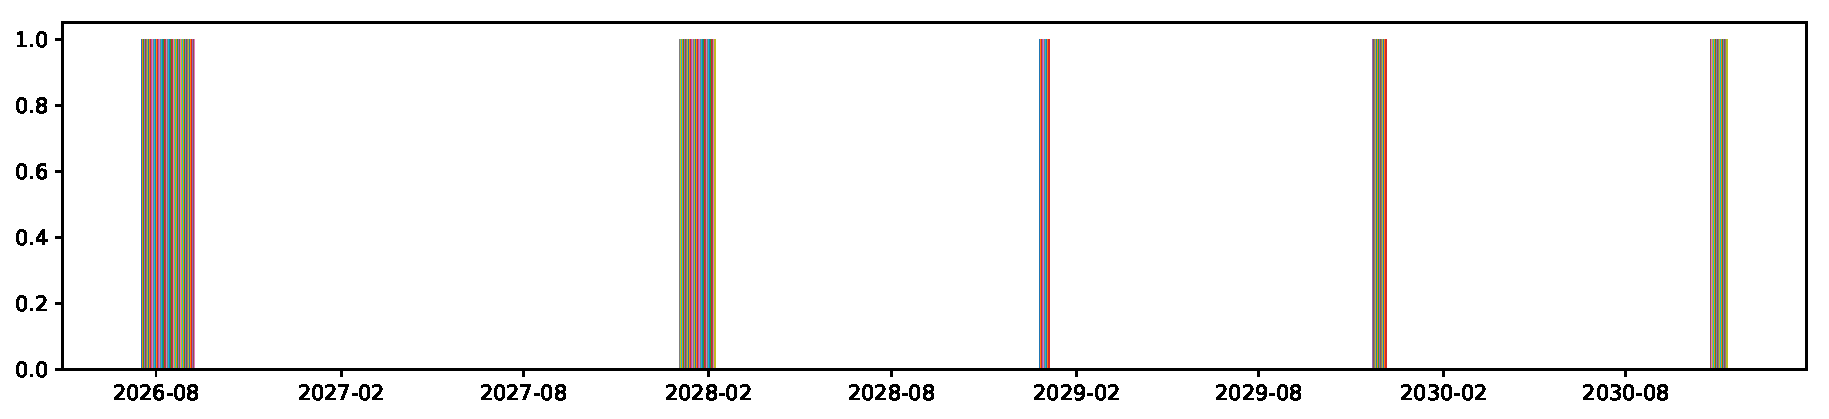
\includegraphics[width=\textwidth]{figures/dates.pdf}
\end{center}
\caption[]{
Dates of observations (is this useful? hard to make it readable)
\label{fig:dates}}
\end{figure*}

\begin{figure}
\begin{center}
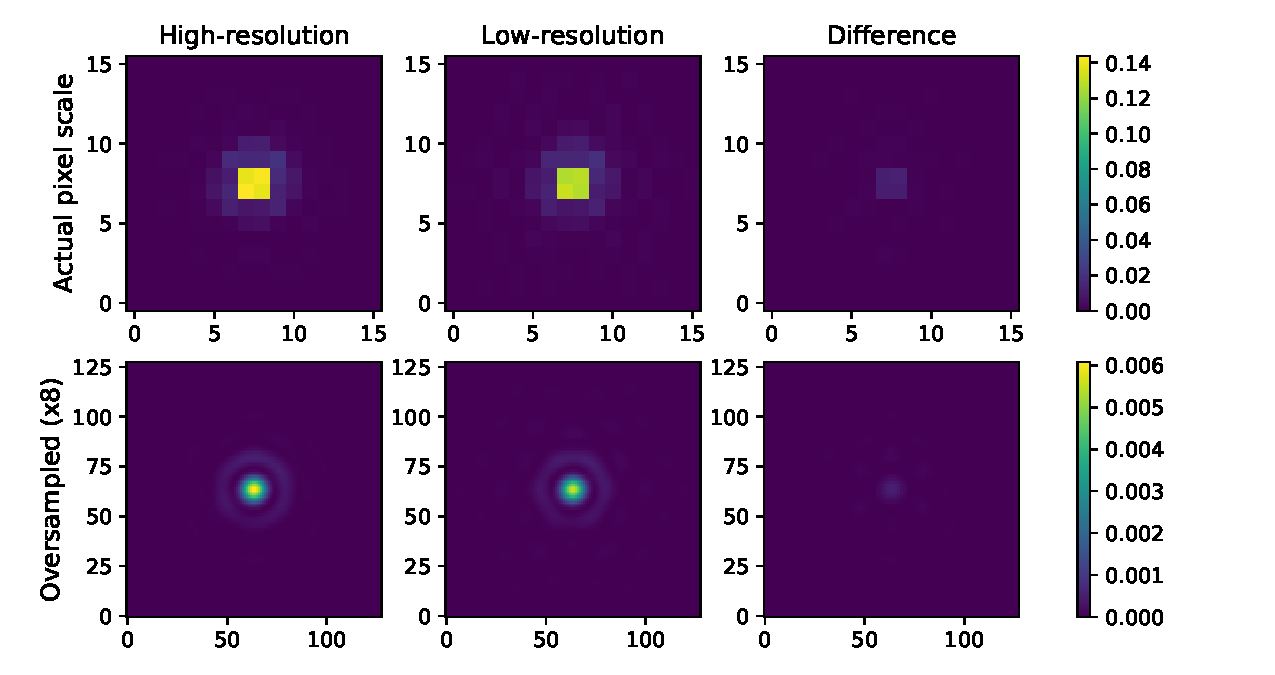
\includegraphics[width=\columnwidth]{figures/psf.pdf}
\end{center}
\caption[]{
PSF model for SCA 1. The top row shows the model in native pixel scale, while the bottom row is oversampled by a factor of 8. From left to right: a comparison of the high-resolution ('true') model, the low-resolution model used in the simulation, and the difference of the two models. The color bars are defined by the range of the high-resolution model.
\label{fig:psf}}
\end{figure}


\section{Simulation suite}\label{sec:sim}

\begin{itemize}
\item We have developed a realistic synthetic survey 
\item into to a synthetic survey and necessary components
\item galsim framework and cycle 7 (\verify{6?}) baseline
\item Detailed description of simulation suite components
\end{itemize}

To empirically test weak lensing requirements, methods, and algorithms in WFIRST, we have designed a sufficiently complex synthetic survey that, while not entirely realistic in all object properties, contains sufficiently complex and representative objects as to enable informative tests and preliminary algorithm development. 
This synthetic survey utilizes several external simulation and data sources, and generates WFIRST-like imaging using the GalSim framework and its WFIRST module. 
The simulation framework is generally capable of producing a full WFIRST HLS imaging survey in all filters matching Cycle 7 specifications. 
The code is publicly available at \url{https://github.com/matroxel/wfirst_imsim}, where configuration files are provided for the fiducial simulation used in this work.
Figure \ref{fig:fov} shows an example pointing produced in the fiducial simulation, and Fig. \ref{fig:sca} shows a larger view of one of the SCAs. 
Performance details are provided in Appendix \cite{app:performance}. 

\subsection{Simulation stages}\label{stages}

The simulation is broken into several stages:

\textbf{\textit{Truth catalog generation}} -- A truth catalog is generated from the input galaxy distribution, photometric galaxy catalog, and Milky Way simulation. 
The following true object properties are assigned to each galaxy in the input galaxy distribution (from which the unique galaxy id is generated): 
1) The position in RA and Dec from the galaxy distribution; 
2) Photometric properties drawn from a random object in the photometric galaxy catalog (consistent $YJHF$ magnitudes, size, and redshift); 
3) Intrinsic ellipticity components drawn from a Gaussian distribution of width 0.27 (truncated at $\pm$0.7); 
4) A random rotation angle; 
5) The ratio of fluxes in each of the three galaxy components: a) de Vaucouleurs bulge, b) exponential disk, and c) random walk star-forming knots (a maximum of 25\% of flux can exist in the knots); 
6) The gravitational shear applied to the object, drawn from a discrete list of $(e_1, e_2) \in \{\pm 0.1, \pm 0.1\}$, though including a coherent shear field instead is a simple modification. 
Further details on the provenance of the galaxy catalogs and Milky Way simulation can be found in Secs. \ref{galcats} and \ref{starcat}, respectively. 
These truth properties are saved in a light-weight FITS format that is accessed by the following stages.

\textbf{\textit{Image generation}} -- In this stage, an empty SCA image is initialized ($4088\times4088$ pixels), and a model is built for each galaxy and star is turn, then drawn into the image. 
The galaxy models are built chromatically from the truth parameters for the object, with each component being assigned a different representative SED of types: S0 (bulge), SBa (disk), and Im (knots), respectively. 
The assigned SED is the same for all objects, since after redshifting the spectrum and applying the appropriate flux in each component and size, the model is converted to be achromatic in each passband to speed up the drawing.\footnote{This simplification can be removed, however, at the cost of multiple factors of increased runtime.}
The intrinsic ellipticity, random rotation, and gravitational shear is then applied.
For stars, we apply the SED of Alpha Lyra to a chromatic delta function model. 
Stars are also converted to be achromatic before drawing.
Both stars and galaxies are then convolved with the appropriate PSF for the SCA (constant across the SCA in the fiducial simulation). An example of the PSF model for an object is shown in Fig. \ref{fig:psf}. We save images of the true PSF model both at native pixel scale and oversampled by a factor of 8, in stamps of native pixel size $8\times 8$ at the position of each galaxy.

The models are drawn in dynamically-sized squares stamps, the sizes of which are chosen automatically by GalSim to include at least 99.5\% of the flux.
These stamps are then added to the SCA image and saved separately (if drawing a galaxy) to provide an isolated image of each simulated galaxy to allow for tests of the impact of blending.
Objects that would have a postage stamp that overlaps the SCA image are drawn, such that light from objects in chip gaps are appropriately drawn onto the SCA, but we only save postage stamps for objects that have a centroid that falls on the SCA. 
We do not save isolated postage stamps of objects that have a stamp size of greater than 288$\times$288 pixels, but they are drawn into the images.
Finally, each isolated postage stamp is processed through the steps described in Sec. \ref{effects} to simulate the WFIRST observatory and detectors and written to disk. When all objects are added to the full SCA image, it is also processed through these steps and written to a FITS image file.
The simulation is parallelized at the SCA level, such that each SCA in each pointing can be run independently. 
(send sentence to appendix) The truth file is lightweight and completion time semi-random, such that even remote disk I/O has not been a limiting factor at the level of thousands of parallel jobs. 

\textbf{\textit{MEDS creation}} -- We then compile the output across pointings of the isolated object stamps into MEDS (Multi-Epoch Data Structure) files\footnote{https://github.com/esheldon/meds}. 
These files concatenate all exposures of unique objects to allow for fast access for object-by-object data processing (like shape measurement). 
Each MEDS file also stores for each object (and stamp) its original SCA, the object position and the stamp position within the SCA, the WCS for each stamp, the PSF model for each object, and other ancillary information. 
Each MEDS file contains all objects within a $n_{\textrm{side}}=512$ Healpixel.

\textbf{\textit{Shape measurement}} -- We utilize the MEDS files to measure the shapes of each galaxy and the PSF. 
The galaxy shape is measured by jointly fitting a two-component model, de Vaucouleurs bulge and exponential disk, across all suitable exposures. 
Exposures where more than 20\% of the pixels are masked (i.e., the centroid falls too close to the edge of the SCA) are rejected. 
The model fit has x parameters: $e_{1,2}$, $p_{x,y}$, half-light radius, flux, and bulge flux fraction, where $e_{1,2}$ is the component of the ellipticity and $p_{x,y}$ is the pixel centroid offset. 
The fits are done using the \textsc{ngmix}\footnote{https://github.com/esheldon/ngmix} and \textsc{MOF}\footnote{https://github.com/esheldon/mof} packages \cite{2014MNRAS.444L..25S}. 
We also measure the PSF size and shape using an adaptive moments method \cite{2003MNRAS.343..459H}. 
This stage writes a set of FITS files containing the galaxy and PSF measurement results and relevant truth catalog information.

\subsection{GalSim}



\subsubsection{Implemented detector effects}\label{effects}


\subsection{Galaxy catalogs}\label{galcats}

The input galaxy catalog is created using a simulated galaxy distribution on the sky taken from one realization of the Buzzard simulation \cite{2019arXiv190102401D,wechsler2019}, to introduce realistic galaxy clustering. Each galaxy is then assigned a random set of photometric properties matching a galaxy from a sample based on the Candels survey that simulates the fiducial WFIRST weak lensing sample selection \cite{2019ApJ...877..117H}. We show the galaxy distribution in Fig. \ref{fig:galaxies}. We use a galaxy density that is approx. 40 arcmin$^{-2}$. In Fig. \ref{fig:hist}, we show the distributions of size, redshift, and H158 magnitude in the Candels sample. We discard less than 1\% of the largest objects in the shape measurement stage, however, due to a maximum postage stamp size restriction. In general, the input distribution and properties of galaxies can be easily modified by configuration (i.e., specifying a different input galaxy catalog).

\verify{Need lensing selection cuts and maybe short description of candels sample.}

\subsection{Star catalog}\label{starcat}

We simulate the positions and magnitudes in WFIRST bandpasses of input stars using the galaxy simulation Galaxia\footnote{http://galaxia.sourceforge.net} \cite{galaxia}. Galaxia uses an analytic model \cite{galaxia2}  to simulate stars in the galaxy that includes a thin and thick disk with warp and flaring, bulge, and halo components. Stars are simulated to 27th magnitude in V band, extinction is added, and they are uniformly translated to WFIRST bandpasses using the stellar SED of Alpha Lyra derived from HST CALSPEC and packaged with GalSim. 

\subsection{Survey strategy}
\assign{Hirata}

\subsection{Simulation implementation for this study}

In this work, we are interested in the impact of how a variety of biases in the PSF model propagate to shape measurement and the weak lensing signal. To study this, we produce a set of 13 image simulations that are identical, including noise, modulo a single PSF model change relative to the fiducial simulation in each case. The details of these changes and their impacts are described in more detail in Sec. \ref{results}. Shape measurement is then performed on the images with some PSF model bias, but using the fiducial, unbiased PSF model for deconvolution, to simulate an unknown wavefront error .

Several simplifications are employed relative to the generic synthetic survey generation described in Sec. \ref{stages} to accommodate the computational load of the many realizations of the survey we are producing. 
\begin{itemize}
\item We simulate objects in a 2.5$\times$2.5 deg$^2$ patch of the sky.
\item We only simulate pointings targeted for the H158 filter. 
Since we are not simulating chromatic effects, the specific filter choice does not make a large difference in our results. 
\verify{This will have an impact on the 'averaging' of PSF errors, however, ...need justification or explanation} 
\item We use a lower-resolution version of the PSF, which significantly speeds up the convolution.
The impact of this approximation on the PSF model, in both native and oversampled pixels, can be seen in Fig. \ref{fig:psf}. 
\item To better isolate the effects of PSF changes, we only utilize the isolated object postage stamps in shape measurement.
\item We do not simulate objects with photometry that would fall below the fiducial weak lensing selection criteria.
\item We do not implement a shear calibration scheme like metacalibration, since we only care about changes to the recovered shape between simulation runs.
\end{itemize}

We simulate a total of 907,170 unique galaxies and 56,128 unique stars across 189 pointings in each of the runs. The distribution of PSF properties and exposures per galaxy are shown in Fig. \ref{}.

\section{Impact of wavefront errors}\label{sec:results}

\begin{itemize}
\item background on psf and wavefront errors
\item details of wfirst psf in cycle 7 (\verify{6?}) baseline
\item summary of approach 
\end{itemize}

In this paper, we focus on empirical tests of weak lensing requirements for wave front model control (i.e., the PSF) in WFIRST. 

\subsection{Static biases}\label{sec:static}

Describe static bias cases

\subsection{High-frequency biases}\label{sec:low}

Describe high-frequency bias cases

\subsection{Low-frequency biases}\label{sec:high}
\assign{Long}

Describe low-frequency bias cases

\subsection{results}\label{sec:results}

present results in some way

\section{Conclusion}\label{sec:conclusion}

wrap-up

future work and timeline

\section*{Acknowledgements}

This work used resources on the CCAPP condo of the Ruby Cluster at the Ohio Supercomputing Center \cite{OhioSupercomputerCenter1987} and ...OSG, Duke.... Plots in this manuscript were produced partly with \textsc{Matplotlib} \cite{Hunter:2007}, and it has been prepared using NASA's Astrophysics Data System Bibliographic Services.

\bibliographystyle{apsrev4-1}
\bibliography{short}

\label{lastpage}

\end{document}
